\documentclass{article}
\usepackage[utf8]{inputenc}
\usepackage[francais]{babel}
\usepackage[T1]{fontenc}
\usepackage{tikz}
\usepackage{graphicx}
\usepackage[left=2cm,right=2cm,top=2cm,bottom=2cm]{geometry}

\title{Rapport du projet de programmtion 2}
\author{Jules Kozolinsky, Gabriel Lebouder, Julien Rixte}

\begin{document}
\maketitle

\section{Introduction}
Dans ce projet, nous avons du coder un jeu de type tower defense. Nous avons donc choisi de mettre en scène la protection d'une vallée contre des vagues de monstres ennemis. Pour cela, le joueur pourra construire des tours au dessus de la vallée afin de s'assurer que les monstres ne la traversent pas. 
\par
Nous avons subdivisé notre code en différents packages traitant chacun d'un aspect du problème. Nous expliquerons dans un premier temps le fonctionnement du jeu. Puis, nous présenterons les interactions entre nos packages. Enfin, nous verrons plus en détail l'organisation de chaque package.

\section{Fonctionnement du jeu}
Le jeu se déroule en différents niveaux. À chaque niveau, le joueur se voit attribuer un montant d'or et un nombre de vies. L'or permet de créer des tours. Le nombre de vies diminue lorsque des monstres parviennent à passer les défenses érigées par le joueur. Lorsque le joueur n'a plus de vie, il a perdu$_{the game}$.
\par
Chaque niveau consiste en une série de vagues de monstres précédées chacune d'une phase de positionnement défensif. Lors de la phase de positionnement, le joueur peut placer des tours de défense dans la limite de l'or disponible. Ces tours peuvent être de plusieurs type et certaines, bien que plus puissantes, peuvent coûter plus cher que d'autres. Une fois le positionnement effectué, le joueur peut lancer la vague de monstres en cliquant sur le bouton play.
\par
Les monstres vont alors essayer de passer outre les défenses du joueur. Chaque monstre tué rapporte un montant d'or proportionnel à la difficulté à tuer celui-ci. Pendant cette phase de jeu, il est impossible d'ajouter les tours. C'est pourquoi nous avons ajouté un bouton d'avance rapide permettant d'accélérer le jeu.
\par
À la fin du jeu, il suffit de cliquer sur l'image indiquant la défaite ou la victoire du joueur pour recommencer une partie.

\section{Interactions entre nos packages}
Nous avons choisi de diviser le code en trois parties principales : l'interface graphique (\textbf{gui}), le contrôle du jeu (\textbf{game}) et la carte (\textbf{map}). L'idée derrière cette organisation était de cloisonner le plus possible différentes parties du codes afin qu'elles puissent fonctionner indépendemment. 
\par
Ainsi, afin que l'interface graphique puisse être changée aisément, aucun élément ayant trait à \textbf{gui} n'apparaît dans les autres parties du code. Pour cela, gui ne fait que lire les informations de \textbf{map} pour afficher les éléments de la carte et demande à \textbf{game} de s'actualiser lorsque cela est nécessaire. 
\par
Le package game interroge le package map. La carte se charge du déplacement physique des monstres et de l'emplacement des tours. Ainsi ce sera le package \textbf{map} qui déterminera s'il est possible de placer une tour à une position donnée, et mais aussi de la position où le monstre doit se déplacer. La \textbf{map} dispose en effet d'une carte des monstres et des tours, alors que \textbf{game} dispose uniquement d'un \textit{Set} de monstres. 
\par
Une quatrième partie, \textbf{entities}, qui correspond à la configuration des tours et des monstres, dispose de classes permettant de créer facilement de nouveaux types de tours ou de monstres. C'est dans cette partie que les caractéristiques des différents objets (monstres et tours) sont définis, ainsi que les types correspondants. Le package entities définit les fonctions apply des objets qui appellent le package map pour trouver les monstres dans le cas des tours, les cases de progression dans le cas des monstres.


\begin{figure}[h]
\center
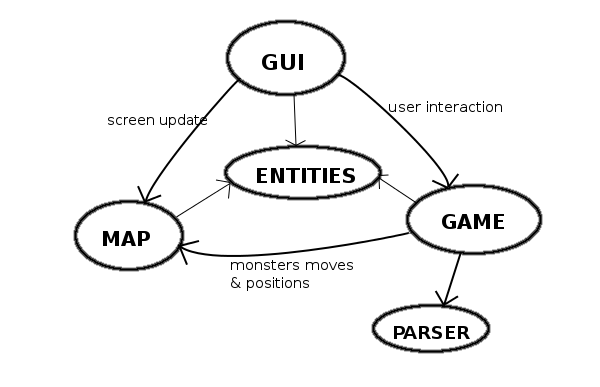
\includegraphics[scale = 0.4]{interactions.png}
\caption{Interactions entre les packages}
\end{figure}



\section{Les différents packages}

\subsection{Entities}
Cette partie contient les définition des objets qui vont évoluer sur la map.\\
Ils sont subdivisés en classes comme montré ci-haut.\\
Les classes apparaissant plus haut sont toutes abstraites, on trouve en feuilles des arbres les classes instanciables (Tower1, Tower2, Monster5, Tower1Type, Monster6Type...).\\
Les classes instanciables se finissant en Type sont des objects.


\begin{figure}[h]
\center
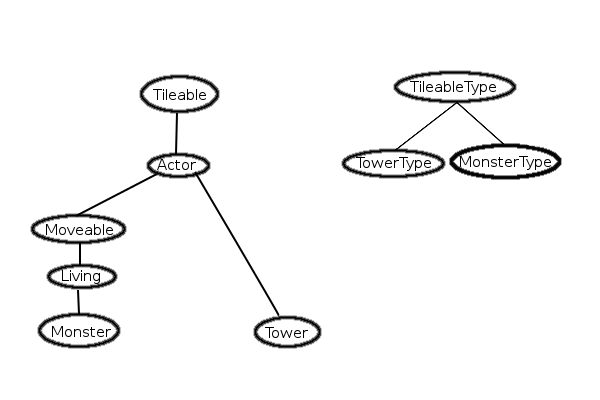
\includegraphics[scale = 0.4]{Entities.png}
\caption{Les différents niveaux d'entitées}
\end{figure}

\subsection{Game}
C'est dans ce package qu'est géré le déroulement interne du jeu. C'est 
\subsubsection{Round}
Le package round gère les actions faites à chaque tick du timer par les tours et les monstres, il dispose pour cela d'un set de monstres et des vagues susceptibles d'arriver sur la map. C'est lui qui appelle les apply des tours et monstres.
\subsubsection{Level}
Le package level est celui qui est appelé par gui, c'est lui qui relance round en permanence et qui gère les cas d'arrêt de jeu.
\subsection{Parser}
Le package \textbf{parser} s'occupe d'extraire d'un fichier XML les différentes informations sur un \textit{Level}, par exemple le nombre de round ou encore la date à laquelle les monstres de différents types vont apparaître, i.e. toutes les informations nécessaires pour construire un \textit{Level}. En pratique le \textbf{parser} ne fonctionne pas à cause d'un problème dûe à la librairie d'extraction de XML. On écrit donc naïvement à l'intérieur du package pour implémenter nos exemples. 

\subsection{Map}
Le package \textbf{map} représente les emplacements physiques des entités du jeu. En réalité, il existe trois cartes différentes : \textit{ground} représentant les obstacles fixes du jeu (par exemple des roches, des arbres ou encore des rivières), \textit{towers} représentant la position des différentes tours et \textit{monsters} représentant la position des monstres pendant un round. Ces trois cartes étant \textit{privées}, les autres packages \textbf{game} et \textbf{gui} appellent des fonctions particulières du package, par exemple s'il est possible de placer une tour, ou pour avoir accès aux monstres situés à une position donnée, ou également pour connaître la prochaine position d'un monstre. 
\par
En effet c'est le package \textbf{map} qui se charge de calculer le déplacement des monstres (pour l'instant naïvement dans la vallée). 


\subsection{Gui}

\begin{figure}[h]
\center
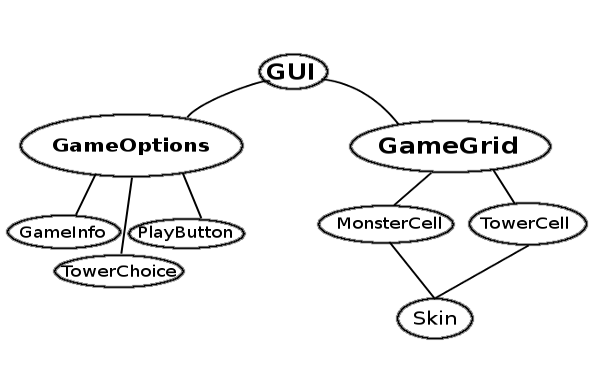
\includegraphics[scale = 0.4]{schema_gui.png}
\caption{Organisation de GUI}
\end{figure}

Le package \textbf{gui} contient l'interface graphique du jeu. Celle-ci a été écrite avec swing. L'objet principal est \textit{MainFrameGUI}. Il contient notamment la fonction actualize qui permet d'actualiser complètement \textbf{gui}. L'interface est alors séparée en deux parties : \textit{GameOptions} qui contient les options du jeu, situées en haut et \textit{GameGrid} qui contient la grille du jeu. \textit{GameOptions} est principalement constitué de boutons et d'informations sur le jeu. \textit{GameGrid} est le coeur de l'interface. C'est une grille qui peut contenir des \textit{MonsterCell} ou des \textit{TowerCell}. La fonction actualize de \textit{GameGrid} est la principale fonction d'actualisation de l'interface : c'est elle qui va lire la carte afin de placer les monstres et les tours à leur place.
\par
La gestion des images a posé de nombreux problèmes : en effet, nous n'avons pas trouvé d'autre moyen que de recharger le fichier image pour changer ses dimensions. Nous avons donc essayé de minimiser le nombre de fois où l'on change de taille d'image. De cette idée est née la classe \textit{Skin} qui permet un partage d'image entre les différentes entités de la grille et une évaluation paresseuse des différentes échelles dont on a besoin pour l'image. Cette classe permet donc de mettre autant de monstres qu'on le souhaite sur une même case sans pour autant ralentir de manière significative.


\section{Ce qu'on aimerait faire}
\begin{itemize}
\item Wave serait une classe comprenant des entiers : hour-to-start ; nmber-of-monster1 ... ; ... nmber-of-monster6
\item Un fond d'herbe partout sauf sur le chemin des monstres qui serait une sorte de sentier (donc évolutif en fonction de où on pose les tours entre les round, à partir de partie 2)
\item Une matérialisation des tirs des tours (soit des boules qui partent, soit des traits si plus simple)
\item Le numéro du round qui s'affiche dans la gui
\item Des noms plus stylés et des particularités pour les tours : des priority qui diffèrent, possibilité de lancer des boules de feu et donc d'enflammer des monstres (=> les Liveable ont un booléen is-burning initialisé à false) ; FireTower, SpeedyTower, BoomBoomTower (vise tous les monstres sur une case) etc
\item Le nombre de monstres de chaque type s'affiche sur les cases de la gui
\item On n'a plus évolution des tailles de monstres en fonction du nombre de type différents par case
\item On peut upgrader les tours, voire leur ajouter des traits ; on peut aussi les détruire, on récupère des sous mais on perd un peu en tout quand même
\item Un parser qui fonctionne
\item Un Dijkstra en pleine forme
\item Des objets posables même pendant un round, très chers, qui ne tirent pas, rapportent 0 quand détruits, mais qui peuvent faire faire des demi-tour aux monstres et gagner du temps
\item Quand on clique sur une case on a des infos sur ce qui s'y trouve
\item Le parser lit l'argent et le nb de vie en fonction du level pour les mettre dans game
\item Des musiques d'ambiance aléatoires pendant le jeu (GoT, Amélie Poulain, Schrtroumpf, Terminator, Taisez-Vous de Finkelkraut, hymne russe etc...)
\item Gagner plein de sous avec
\item La puissance des tours peut décroître avec la distance
\item La fonction de tri des round ne gère pas encore l'éventualité où deux vagues ont la même date (mais le parser est censé s'en occuper tout seul de toute façon)


\end{document}